\clearpage
\section{数列}
\subsection{二项式系数}
\[\binom nk=\frac{n!}{k!(n-k)!}=\begin{cases}1&\text{for }k=0\\\displaystyle\binom {n-1}k+\binom{n-1}{k-1}&\text{otherwise}\end{cases}\]
\paragraph{生成函数:}
\[\sum_{k=0}^n\binom nkx^k=(1+x)^n\]
\paragraph{性质:}
\begin{itemize}
  \item $\displaystyle\sum_{k=0}^n\binom nk=2^n\qquad\sum_{k=0}^nk\binom nk=n2^{n-1}\qquad\sum_{k=0}^nk^2\binom nk=n(n+1)2^{n-2}$
  \item $\displaystyle\sum_{k=0}^nk^3\binom nk=n^2(n+3)2^{n-3}\qquad\sum_{k=0}^nk^4\binom nk=n(n+1)(n^2+5n-2)2^{n-3}$
  \item Vandermonde 恒等式: $\displaystyle\sum_{k=0}^r\binom mk\binom n{r-k}=\binom{m+n}r$.
    \begin{itemize}
      \item $\displaystyle\sum_{k=0}^{\min\{n,m\}}\binom nk\binom mk=\binom{n+m}{\min\{n,m\}}$
      \begin{itemize}
        \item $\displaystyle\sum_{k=0}^n\binom nk^2=\binom{2n}n$
      \end{itemize}
      \item $\displaystyle\sum_{k=0}^n\binom nk\binom n{k-1}=\binom{2n}{n-1}$
    \end{itemize}
  \item 朱世杰恒等式: $\displaystyle\sum_{k=m}^n\binom kr=\binom{n+1}{r+1}-\binom m{r+1}$
\end{itemize}

关于二项式系数求值的代码在组合排列一节的二项式系数中.

\clearpage
\subsection{自然数等幂和 (Bernoulli 数)}
\[
  \begin{alignedat}{8}
    &\sum_{k=1}^mk^0=&m\\
    &\sum_{k=1}^mk^1=&\frac12m&+&\frac12m^2\\
    &\sum_{k=1}^mk^2=&\frac16m&+&\frac12m^2&+&\frac13m^3\\
    &\sum_{k=1}^mk^3=&&&\frac14m^2&+&\frac12m^3&+&\frac14m^4\\
    &\sum_{k=1}^mk^4=-&\frac1{30}m&&&+&\frac13m^3&+&\frac12m^4&+&\frac15m^5\\
    &\sum_{k=1}^mk^5=&&-&\frac1{12}m^2&&&+&\frac5{12}m^4&+&\frac12m^5&+&\frac16m^6\\
    &\sum_{k=1}^mk^6=&\frac1{42}m&&&-&\frac16m^3&&&+&\frac12m^5&+&\frac12m^6&+&\frac17m^7\\
  \end{alignedat}
\]
设 $\displaystyle\sum_{k=1}^mk^n=\sum_{k=1}^{n+1}b(n,k)m^k$, 有递推式
\[
  b(n,k)=\begin{cases}
    1&\text{for }n=0\land k=1\\
    \displaystyle\frac nkb(n-1,k-1)&\text{for }n>0\land k>1\\
    \displaystyle1-\sum_{k=2}^nb(n,k)&\text{for }n>0\land k=1\\
  \end{cases}
\]
Bernoulli 数即为 $b_n=b(n,1)$.

\begin{lstlisting}[language=Python]
#!/usr/bin/env python3
from fractions import Fraction


def main():
    b = [[0] * 101 for n in range(100)]
    for n in range(10):  # 0 ~ 9
        for k in range(2, n + 2):
            b[n][k] = Fraction(n, k) * b[n - 1][k - 1]
        b[n][1] = 1 - sum(b[n])


if __name__ == '__main__':
    main()
\end{lstlisting}

\clearpage
\subsection{Catalan 数}
\[
  C_n=\frac{2n!}{n!(n+1)!}=\begin{cases}
    1&\text{for }n=0\\
    \displaystyle\frac{2(2n-1)}{n+1}C_{n-1}&\text{otherwise}
  \end{cases}
\]
\paragraph{生成函数:}
\[\sum_{k=0}^\infty C_kx=\frac2{1+\sqrt{1-4x}}\]
\paragraph{含义:}
\begin{itemize}
  \item $C_n$ 表示 $\{1,2,3,\ldots,n\}$ 依序进出栈的置换个数, 下述变种均为等价表述.
  \item $C_n$ 表示长度为 $n$ 的所有合法括号序列.
  \item $C_n$ 表示 $n$ 个节点构成的不同构二叉树个数, 下图月牙为空的情况.
  \item $C_n$ 表示 $2n+1$ 个节点构成的不同构非叶节点满孩子的二叉树个数, 下图月牙为叶子的情况.
    \begin{center}
      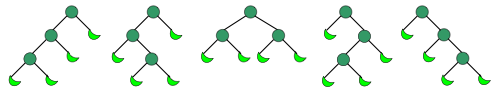
\includegraphics[scale=.5]{SEQ/Catalan_number_binary_tree_example.png}
    \end{center}
  \item $C_n$ 表示在 $n^2$ 格点中不越过对角线的单调路径个数.
    \begin{center}
      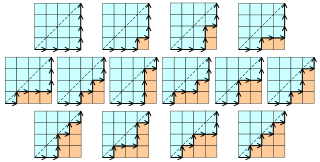
\includegraphics[scale=.5,natwidth=320,natheight=162]{SEQ/320px-Catalan_number_4x4_grid_example.svg.png}
    \end{center}
  \item $C_n$ 表示 $n+2$ 边形划分为三角形方案数.
    \begin{center}
      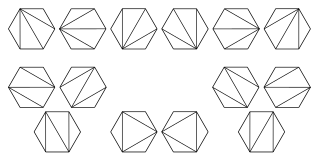
\includegraphics[scale=.5,natwidth=320,natheight=160]{SEQ/320px-Catalan-Hexagons-example.svg.png}
    \end{center}
  \item $C_n$ 表示用 $n$ 个矩形填充一个高 $n$ 的阶梯状图形的方法数.
    \begin{center}
      
\includegraphics[scale=.5,natwidth=320,natheight=85]{SEQ/320px-Catalan_stairsteps_4.svg.png}
    \end{center}
\end{itemize}

\clearpage
\subsection{Stirling 数}
\[
  \begin{aligned}
    s(n,k)&=(-1)^{n+k}\genfrac[]{0pt}0nk&\genfrac[]{0pt}0nk=&\begin{cases}
      1&\text{for }n=0\land k=0\\
      0&\text{for }n=0\lor k=0\\
      \displaystyle(n-1)\genfrac[]{0pt}0{n-1}k+\genfrac[]{0pt}0{n-1}{k-1}&\text{otherwise}
    \end{cases}\\
    S(n,k)&=\genfrac\{\}{0pt}0nk&\genfrac\{\}{0pt}0nk=&\begin{cases}
      1\qquad\qquad\qquad\qquad\qquad\quad\ \ \text{for }n=0\land k=0\\
      0\qquad\qquad\qquad\qquad\qquad\quad\ \ \text{for }n=0\lor k=0\\k
      \genfrac\{\}{0pt}0{n-1}k+\genfrac\{\}{0pt}0{n-1}{k-1}\qquad\quad\!\!\text{otherwise}
    \end{cases}
  \end{aligned}
\]
\paragraph{生成函数:}
\[\sum_{k=0}^ns(n,k)x^k=x^{\underline n}\qquad\sum_{k=0}^nS(n,k)x^{\underline n}=x^n\]
\paragraph{含义:}
\begin{itemize}
  \item $\genfrac[]{0pt}0nk$ 表示 $n$ 个不同元素的集合划分为 $k$ 个不相交子集, 划分内按环排列的方案数.
  \item $\genfrac\{\}{0pt}0nk$ 表示 $n$ 个不同元素的集合划分为 $k$ 个不相交子集的方案数.
\end{itemize}
\paragraph{性质:}
\begin{itemize}
  \item $\displaystyle\sum_{k=0}^n\genfrac[]{0pt}0nk=n!\qquad\sum_{k=0}^n\genfrac\{\}{0pt}0nk=B_n\qquad\triangleright B_n\text{为 ``Bell 数''}$
  \item $\displaystyle\sum_{k=m}^n\genfrac[]{0pt}0nk\binom km=\genfrac[]{0pt}0{n+1}{m+1}\qquad\sum_{k=m}^n\binom nk\genfrac\{\}{0pt}0km=\genfrac\{\}{0pt}0{n+1}{m+1}$
\end{itemize}
\subsection{Bell 数}
\[
  B_{n+1}=\begin{cases}
    1&\text{for }n=0\lor n=1\\
    \displaystyle\sum_{k=0}^n\binom nkB_k&\text{otherwise}\\
  \end{cases}
\]
\paragraph{含义:}
\begin{itemize}
  \item $B_n$ 表示将含有 $n$ 个不同元素的集合划分为不相交子集的方案数.
\end{itemize}
\paragraph{性质:}
\begin{itemize}
  \item $B_{p^m+n}\equiv mB_n+B_{n+1}\pmod p\qquad\triangleright p\text{为素数}$
\end{itemize}

\subsection{Fibonacci 数}
\[
  F_n=\frac{\phi^n+\psi^n}{\sqrt5}=\begin{cases}
    0&\text{for }n=0\\
    1&\text{for }n=1\\
    F_{n-1}+F_{n-2}&\text{otherwise}
  \end{cases}
\]
\paragraph{生成函数:}
\[\sum_{k=0}F_kx^k=\frac x{1-x-x^2}\]
\paragraph{性质:}
\begin{itemize}
  \item $\displaystyle\sum_{k=0}^{\lfloor n/2\rfloor}\binom{n-k}k=F_{n+1}$
  \item $\displaystyle\sum_{k=0}^nF_k=F_{n+2}-1$
  \item $\displaystyle\sum_{k=0}^nkF_k=nF_{n+2}-F_{n+3}+2$
  \item $\displaystyle\sum_{k=0}^nF_{2k}=F_{2n+1}-1$
  \item $\displaystyle\sum_{k=0}^nF_{2k+1}=F_{2n+2}$
  \item $\displaystyle\sum_{k=0}^nF_k^2=F_nF_{n+1}$
  \item Vajda 恒等式: $F_{n+i}F_{n+j}-F_nF_{n+i+j}=(-1)^nF_iF_j$
  \begin{itemize}
    \item Catalan 恒等式: $F_n^2-F_{n-k}F_{n+k}=(-1)^{n+k}F_k^2$
    \begin{itemize}
      \item Cassini 恒等式: $F_{n-1}F_{n+1}-F_n^2=(-1)^n$
    \end{itemize}
  \end{itemize}
  \item d'Ocagne 恒等式:
  \begin{itemize}
    \item $F_mF_n+F_{m-1}F_{n-1}=F_{m+n-1}$
    \begin{itemize}
      \item $F_{2n-1}=F_n^2+F_{n-1}^2$
    \end{itemize}
    \item $F_mF_{n+1}+F_{m-1}F_n=F_{m+n}$
    \begin{itemize}
      \item $F_{2n}=F_n(F_{n-1}+F_{n+1})$
    \end{itemize}
  \item $\displaystyle F_{an+b}=\sum_{k=0}^a\binom akF_{b-k}F_n^kF_{n+1}^{a-k}$
  \end{itemize}
  \item $\gcd(F_m,F_n)=F_{\gcd(m,n)}$
\end{itemize}

\clearpage
\subsection{分拆数}
\[
p(n,k)=\begin{cases}
  1&\text{for }k=1\\
  0&\text{for }k=0\lor k>n\\
  p(n-1,k-1)+p(n-k,k)&\text{otherwise}\\
\end{cases}
\]

\paragraph{生成函数:}
\[\sum_{k=0}^np(n,k)x^k=\prod_{k=1}^n\frac1{1-x^k}\]

\paragraph{含义:} $p(n,k)$ 表示将 $n$ 个数字拆成 $k$ 个数字的和有多少种方式.

利用五边形数 $O(n\sqrt n)$ 初始化所有小于等于自然数 $n$ 的数的分拆数前缀和 $\displaystyle\sum_{k=1}^\infty p(n,k)$.

\begin{lstlisting}
template <typename RandomAccessIt> void
initIntPart(RandomAccessIt p, size_t n) {
  using T = typename iterator_traits<RandomAccessIt>::value_type;
  vector<T> q = {0, 1, 2, 5};
  while (q.back() < n)
    q.push_back(3 + q.end()[-2] * 2 - q.end()[-4]);
  *p = 1; fill(p + 1, p + n, 0);
  for (size_t i = 1; i != n; ++i)
    for (size_t j = 1; q[j] <= i; ++j)
      p[i] += (j + 1 & 2 ? p[i - q[j]] : -p[i - q[j]]);
}
\end{lstlisting}

对于上述问题的变形, 问将自然数 $n$ 拆分成恰好 $k$ 个不同的数的和的方案数, 有递归公式:

\[
p'(n,k)=\begin{cases}
  0&\displaystyle\text{for }k=0\lor k>\frac{\sqrt{8n+1}-1}2\\
  1&\text{for }k=1\\
  p'(n-k,k)+p'(n-k,k-1)&\text{otherwise}\\
\end{cases}
\]

显然, 计算单个 $p'$ 复杂度为 $O(n\sqrt n)$, 计算前 $n$ 个自然数的 $p'$ 均摊复杂度也为 $O(n\sqrt n)$.

\subsection{错排数}
\[
  \begin{aligned}
    D_n=&n!\sum_{k=0}^n\frac{(-1)^k}{k!}\\
    =&nD_{n-1}+(-1)^n\\
    =&(n-1)(D_{n-1}+D_{n-1})\\
    =&\left[\frac{n!}{\mathrm e}\right]\qquad\text{for }n>1
  \end{aligned}
\]

\subsection{Farey 数列}
$n$ 阶 Farey 数列是 0 到 1 之间最简分数组成的数列, 每个分数的分母均不大于 $n$.

代码中的 \lstinline{Rational} 类见杂项有理数.

\lstinputlisting{SEQ/farey.hh}

\subsection{调和级数}
\[H_n=\sum_{k=1}^n\frac1k\]

\paragraph{性质:}
\begin{itemize}
  \item $\displaystyle\lim_{n\to\infty}H_n=\ln n+\gamma$, 其中 $\gamma$ 为 Euler–Mascheroni 常数, 有 (IEEE-754 binary128 精度): \[\gamma\approx0.57721566490153286060651209008240243\]
\end{itemize}
